
\part{Einordnung und Zielsetzung}
%----------------------------------------------------------------------------------------
%	CHAPTER 1
%----------------------------------------------------------------------------------------
\chapterimage{Bilder_und_Co/nasa-erde.jpg} % Chapter heading image
%----------------------------------------------------------------------------------------

\chapter{Aufgabenstellung}
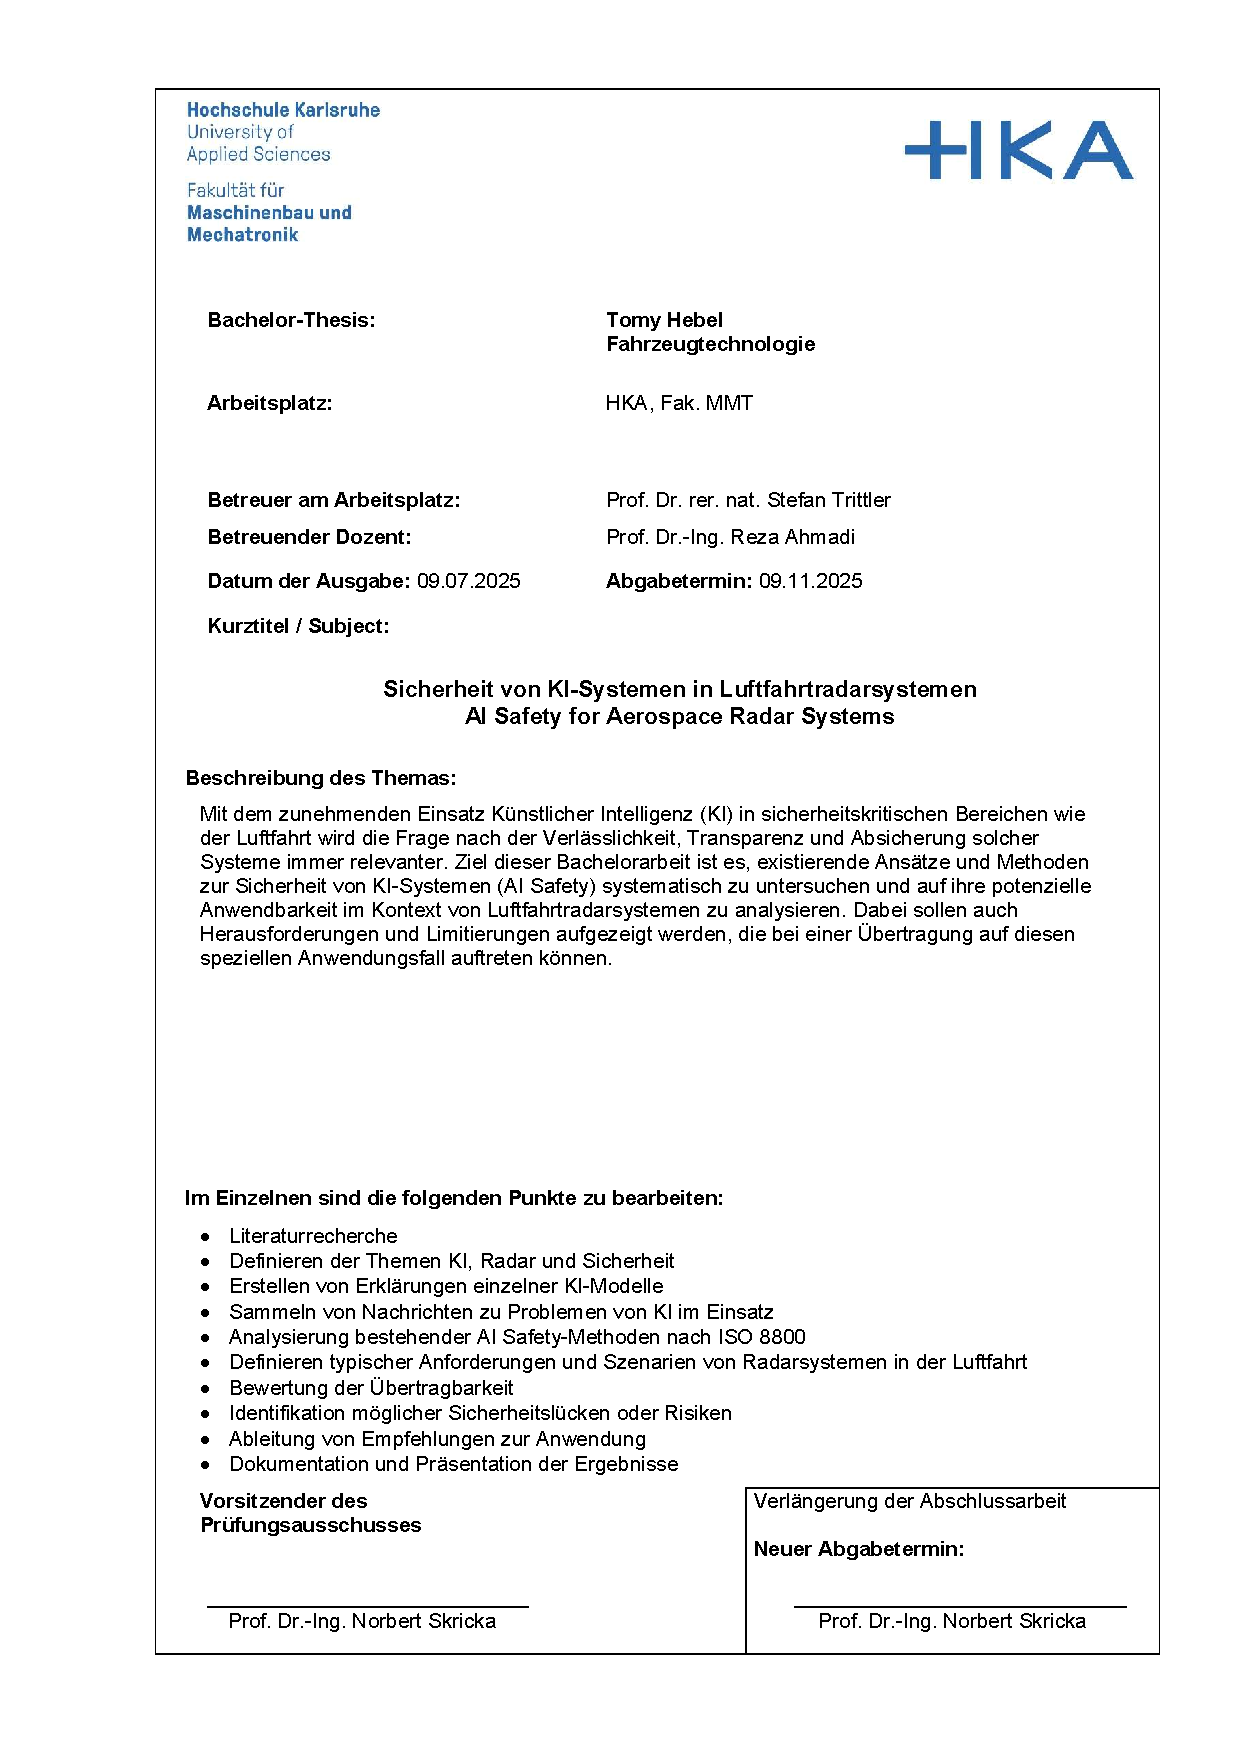
\includepdf[pages=-]{Sicherheit von KI-Systemen in Luftfahrtradarsystemen 09_07.pdf}

\chapter{Einleitung}

\section{Motivation}
Ein Bild, das sich jeder sofort vorstellen kann: Ein Pilot fragt „Hey Siri, wie ist das Wetter?“ 
– die Bordassistenz antwortet: „In 200 km liegt mit 80 \% Wahrscheinlichkeit Starkregen.“ 
Genau daran knüpft diese Arbeit an: Ist KI für solche Funktionen im Flugzeug bereits sicher 
– oder zumindest sicher genug? 

Die zunehmende Integration Künstlicher Intelligenz in technische Systeme eröffnet 
neue Möglichkeiten für Effizienzsteigerungen, Automatisierung und verbesserte 
Entscheidungsunterstützung. Während KI in Bereichen wie der Datenanalyse, der 
Bilderkennung oder der Sprachverarbeitung bereits weit verbreitet ist, stellt 
der Einsatz in sicherheitskritischen Anwendungen eine besondere Herausforderung dar. 
Hierzu zählt insbesondere die Luftfahrt, in der höchste Anforderungen an Zuverlässigkeit, 
Robustheit und Nachweisführung bestehen. Fehler oder Fehlfunktionen haben nicht nur 
ökonomische, sondern vor allem sicherheitsrelevante Konsequenzen.

Ein Bereich, in dem der Einsatz von KI großes Potenzial bietet, sind Radarsysteme 
in der Luftfahrt. Sie sind essenziell für die Detektion und Klassifizierung von 
Objekten, die Wetterbeobachtung und der Navigationsunterstützung. Klassische 
Verfahren stoßen in komplexen oder dynamischen Umgebungen zunehmend an ihre Grenzen, 
sodass KI-basierte Methoden einen Mehrwert in Form verbesserter Erkennungsleistungen 
versprechen.

Gleichzeitig besteht jedoch erhebliche Unsicherheit darüber, ob KI-Systeme den hohen 
Anforderungen der Luftfahrt bereits heute gerecht werden können. Anders als in weniger 
sicherheitskritischen Domänen ist eine Integration ohne umfassende Nachweise nicht denkbar. 
Regulatorische Institutionen wie die EASA haben dies erkannt und erste konzeptionelle 
Leitlinien zur sicheren Entwicklung und Anwendung von KI veröffentlicht. 
Auch etablierte Sicherheitsstandards wie die ISO 8800 aus dem Automotive-Sektor 
bieten einen Referenzrahmen.

Vor diesem Hintergrund gewinnt die Frage nach der Sicherheit von KI-Systemen in 
Luftfahrtradarsystemen zunehmend an Bedeutung -- sind die bestehenden Konzepte und 
Rahmenbedingungen ausreichend, um Vertrauen in die Technologie zu schaffen, 
oder besteht weiterhin wesentlicher Forschungs- und Entwicklungsbedarf, bevor KI 
zuverlässig in sicherheitskritischen Anwendungen eingesetzt werden kann?




\section{Problemstellung}
Im sicherheitskritischen Umfeld der Luftfahrt bleibt offen, ob KI-basierte Systeme 
bereits als hinreichend sicher gelten können. Während KI in vielen Domänen erprobte 
Vorteile zeigt, treffen ihre Nutzungsmöglichkeiten in der Luftfahrt auf besonders 
hohe Anforderungen. Zuständige 
Luftfahrtbehörden adressieren diese Herausforderungen derzeit über konzeptionelle 
Leitlinien. Etablierte Sicherheitsstandards aus anderen Bereichen, wie etwa die ISO 8800 
im Automotive, bieten einen bewährten Bezugsrahmen.

Ungeklärt bleibt jedoch, in welchem Ausmaß vorhandene Konzepte, Vorgehensmodelle 
und Rahmenbedingungen geeignet erscheinen, um Vertrauen in KI-basierte Funktionen zu 
stiften, wenn diese in luftfahrtrelevanten Anwendungen eingesetzt werden. 
Da Radarsysteme sicherheitskritische Komponenten der Luftfahrt sind, lässt 
sich diese Fragestellung exemplarisch an diesem Anwendungsfeld einordnen, 
ohne eine Detailbewertung einzelner Verfahren vorzunehmen. Im Vordergrund steht die 
übergeordnete Einschätzung, welche Ansätze gefordert sind und inwieweit deren 
Abdeckung gegeben ist.

Damit ergibt sich folgendes zentrales Problem: Der aktuelle Stand der Auseinandersetzung 
mit der KI-Sicherheit in der Luftfahrt sowie ihr Reifegrad sind bislang nicht eindeutig 
definiert und eingeordnet. Es ist unklar, inwieweit die bestehenden Konzepte und 
Rahmenbedingungen ausreichen, um Vertrauen in KI-basierte Funktionen in sicherheitskritischen 
Anwendungen der Luftfahrt zu begründen.


\section{Forschungsfrage}
Ist der Einsatz von KI in Luftfahrtradarsystemen 
unter den aktuell verfügbaren Sicherheitskonzepten und regulatorischen Rahmenbedingungen 
als hinreichend sicher zu betrachten?

\subsection*{Weitere Fragen}
Luftfahrtforderungen:\\
Welche Anforderungen und Leitlinien werden derzeit von 
luftfahrtspezifischen Institutionen wie EASA an KI-Sicherheit gestellt?

\medskip
Maßnahmen etablierter Standards:\\
Welche Maßnahmen werden von etablierten internationalen Standards wie die ISO 8800 aus der Automotivebranche 
an die Sicherheit von KI-Systemen definiert?

\section{Ziel und Beitrag der Arbeit}
Ziel dieser Arbeit ist es, die Forschungsfrage zu beantworten.
Hier gilt es anhand der hohen Anforderungen der Luftfahrt zu prüfen, in welchem Umfang 
diese durch aktuelle Standards adressiert werden.
Das Ergebnis soll eine Einordnung liefern, in welchen Bereichen die vorhandenen Konzepte und 
Rahmenbedingungen bereits Vertrauen in KI-basierte Funktionen ermöglichen und wo weiterer 
Forschungs- und Entwicklungsbedarf besteht.

\medskip
Die Arbeit leistet eine strukturierte Zuordnung zwischen (I) den in 
etablierten Sicherheitsstandards sowie behördlichen Leitlinien geforderten 
Absicherungsansätzen und (II) der erkennbaren Abdeckung durch heutige 
Vorgehensweisen im Radar-Kontext. Daraus resultieren:

\medskip
\begin{itemize}
\item eine konsolidierte Anforderungs- und Coverage-Matrix (Forderung~$\leftrightarrow$ Abdeckung~$\leftrightarrow$ Begründung)
\item eine verdichtete Übersicht typischer Lücken und Risiken
\item empfehlungsorientierte Schlussfolgerungen für Anwendung und Weiterentwicklung
\end{itemize}



% Spaltenabstand (zwischen den Spalten) einstellbar:
\newlength{\colsepA}\setlength{\colsepA}{8mm}

% SpaltenBREITEN bequem als Längen steuerbar:
\newlength{\colL}\setlength{\colL}{0.14\textwidth} % linke Labelspalte
\newlength{\colA}\setlength{\colA}{0.3\textwidth} % Automotive
\newlength{\colB}\setlength{\colB}{0.48\textwidth} % Luftfahrt

\begin{table}[h]
\centering
\caption{Erläuterung der Ausgangslage dieser Arbeit}
\renewcommand{\arraystretch}{1.2}
\begin{tabular}{
  @{} p{\colL}
  @{\hspace{\colsepA}}
  >{\centering\arraybackslash}p{\colA}
  @{\hspace{\colsepA}}
  >{\centering\arraybackslash}p{\colB}
  @{}
}
\toprule
\textbf{} & \textbf{Automotive} & \textbf{Luftfahrt} \\
\midrule
\textbf{Anforderungen an KI}
&
*(Welche Anforderungen stellt die Automobilbranche an die Sicherheit von KI?)
&
Welche Anforderungen formulieren Luftfahrtbehörden wie EASA an die KI-Sicherheit? \\
\midrule
\textbf{Maßnahmen / Standards zu KI}
&
Welche Maßnahmen definieren etablierte Standards wie ISO\,8800 zur Absicherung von KI?
&
Da für die Luftfahrt bislang keine eigenständigen KI-Sicherheitsstandards etabliert sind, wird geprüft, inwieweit die luftfahrtspezifischen Anforderungen durch Maßnahmen aus der Automotive abgedeckt werden können. \\
\bottomrule
\end{tabular}
\label{tab:ausgangslage}
\end{table}

* (Nicht Teil der Arbeit.)







\subsection*{Abgrenzung}
Nicht Gegenstand dieser Arbeit ist die Detailbewertung oder 
Zertifizierung einzelner Algorithmen oder Produkte.
Radarsysteme dienen als Anwendungsrahmen; weitere Einsatzmöglichkeiten von KI in 
der Luftfahrt werden berücksichtigt, jedoch nicht vertieft. Zur Veranschaulichung 
werden ausgewählte Beispiele punktuell herangezogen (etwa KI-gestützte Mustererkennung 
im Entwicklungs-/Nachweisprozess), ohne daraus eine generelle Aussage zur 
Inline-Integration abzuleiten. Die Arbeit setzt auf publizierte Quellen und 
öffentlich zugängliche Leitlinien.



\section{Vorgehensweise}
Im Verlauf dieser Arbeit wird folgendermaßen vorgegangen:

\medskip
Es wurden Literaturrecherchen zu AI-Safety, Luftfahrtsicherheit und Radar gemacht, 
die mittels Grundlagen gestützt werden. 

Hinzu kommt eine Sammlung ausgewählter Praxisberichte von KI im Einsatz. Weiter werden 
möglicher Sicherheitslücken und Risiken identifiziert und Erkenntnisse aus der Praxis betrachtet.

Es wird ein Abgleich geforderter Ansätze mit der heutigen Abdeckung untersucht. 
Zudem wird zur besseren Darzustellung dies anhand eines Beispieles verdeutlicht wofür
Anforderungen und Szenarien für ein Radarsystem definiert und die Übertragbarkeit bewertet wird.

Schließlich werden die so gewonnenen Erkenntnisse Zusammengetragen und Empfehlungen abgeleitet.



\newpage
\begin{figure}[h!]
\centering
\begin{tikzpicture}[
  node distance=18mm and 18mm,
  box/.style={draw, rounded corners, align=center, text width=32mm, minimum height=8mm, fill=gray!5},
  arrow/.style={-{Latex}, thick},
  markpos/.style={label position=north east, label distance=-2pt},
  marknode/.style={draw, circle, inner sep=0.2ex, minimum size=1.6ex, line width=0.3pt, font=\scriptsize, fill=white}
]

% --- Obere Reihe ---
\node[box, markpos, label={[marknode]north east:{\textbf{1}}}] (auto) {\nameref{chap:automotiv}};
\node[box, right=of auto, xshift=-12mm, markpos, label={[marknode]north east:{\textbf{2}}}] (ref) {\nameref{chap:referenz}\\};
\node[box, right=of ref, xshift=-12mm, markpos, label={[marknode]north east:{\textbf{3}}}] (radar) {\nameref{chap:szenarien}};
\node[box, right=of radar, xshift=-12mm, markpos, label={[marknode]north east:{\textbf{4}}}] (models) {\nameref{chap:modelle}};

% --- Zweite Reihe ---
\node[box, below=of auto, yshift=5mm, markpos, label={[marknode]north east:{\textbf{5}}}] (iso) {\nameref{chap:iso-8800}};
\node[box, below=of ref, yshift=5mm, xshift=5mm, markpos, label={[marknode]north east:{\textbf{6}}}] (avi) {Luftfahrt-\\rahmen-\\bedingungen}; %\nameref{chap:anf-avi}
\node[box, below=of radar, yshift=7mm, xshift=15mm, markpos, label={[marknode]north east:{\textbf{7}}}] (anfref) {\nameref{chap:anforderungen}\\ (Anforderungen)};

% --- Dritte Reihe ---
\node[box, below=of avi, xshift=-15mm, markpos, label={[marknode]north east:{\textbf{8}}}] (cov) {\nameref{chap:coverage}};
\node[box, below=of anfref, yshift=7mm, xshift=-18mm, markpos, label={[marknode]north east:{\textbf{9}}}] (zuord) {\nameref{chap:anforderungen}\\ (Zuordnung)};

% --- Vierte Reihe ---
\node[box, below=of cov, xshift=23mm, markpos, label={[marknode]north east:{\textbf{10}}}] (ueber) {\nameref{chap:uebertragbarkeit}};

% --- Fünfte Reihe ---
\node[box, below=of ueber, yshift=6mm, markpos, label={[marknode]north east:{\textbf{11}}}] (empf) {\nameref{chap:empfehlungen}};


% --- Pfeile ---
\draw[arrow] (auto) -- (iso);
\draw[arrow] (ref) -- (avi);
\draw[arrow] (radar) -- (anfref);
\draw[arrow] (models) -- (anfref);
\draw[arrow] (iso) -- (cov);
\draw[arrow] (avi) -- (cov);
\draw[arrow] (avi) -- (zuord);
\draw[arrow] (anfref) -- (zuord);
\draw[arrow] (zuord) -- (ueber);
\draw[arrow] (cov) -- (ueber);
\draw[arrow] (ueber) -- (empf);

\end{tikzpicture}
\caption{Illustration des Aufbaus der Arbeit: Kapitelbezüge und Datenfluss.}
\end{figure}


Zunächst werden die notwendigen Grundlagen zu KI, Radarsystemen und Sicherheit
skizziert.
Darauf aufbauend folgt eine Einordnung des heutigen KI-Einsatzes zusammen mit 
Herausforderungen und Risiken.
Anschließend werden Referenzrahmen \textbf{2} aufgeführt und die luftfahrtspezifischen 
Rahmenbedingungen\textbf{6} genauer betrachtet. 
Hinzu kommt ein Vergleich der Automobil- und Luftfahrtbranche \textbf{1} mit Blick auf 
KI spezifissche Sicherheitsanforderungen mit einer vertiefung zu jüngst eingeführten 
Automobilstandards \textbf{5}. 
Die so identifizierten allgemeinen Luftfahrtanforderungen werden den
Automobilstandards gegenübergestellt, um Übereinstimmungen und Lücken mittels einer \nameref{chap:coverage} \textbf{8} aufzuzeigen.
Für eine konkrete Beispielbetrachtung wird anschließend ein Radarsystem \textbf{3} samt
Einsatzzweck sowie ein KI-Modell \textbf{4} mit passender Funktion gewählt; hierfür werden spezifische
Anforderungen \textbf{7} definiert und mit luftfahrtspezifischen Referenzrahmen 
abgeglichen \textbf{9}. 
Die Abdeckung der Beispielanforderungen wird daraus abgeleitet \textbf{10}.
Anschließend werden und Empfehlungen \textbf{11} formuliert. Den Abschluss bildet ein
Fazit mit den zentralen Erkenntnissen.

